\documentclass{beamer}
\usepackage[utf8]{inputenc}

\usetheme{Madrid}
\usecolortheme{default}
\usepackage{amsmath,amssymb,amsfonts,amsthm}
\usepackage{txfonts}
\usepackage{tkz-euclide}
\usepackage{listings}
\usepackage{adjustbox}
\usepackage{array}
\usepackage{tabularx}
\usepackage{gvv}
\usepackage{lmodern}
\usepackage{circuitikz}
\usepackage{tikz}
\usepackage{graphicx}
\usepackage{mathtools}
\setbeamertemplate{page number in head/foot}[totalframenumber]

\usepackage{tcolorbox}
\tcbuselibrary{minted,breakable,xparse,skins}



\definecolor{bg}{gray}{0.95}
\DeclareTCBListing{mintedbox}{O{}m!O{}}{%
  breakable=true,
  listing engine=minted,
  listing only,
  minted language=#2,
  minted style=default,
  minted options={%
    linenos,
    gobble=0,
    breaklines=true,
    breakafter=,,
    fontsize=\small,
    numbersep=8pt,
    #1},
  boxsep=0pt,
  left skip=0pt,
  right skip=0pt,
  left=25pt,
  right=0pt,
  top=3pt,
  bottom=3pt,
  arc=5pt,
  leftrule=0pt,
  rightrule=0pt,
  bottomrule=2pt,
  toprule=2pt,
  colback=bg,
  colframe=orange!70,
  enhanced,
  overlay={%
    \begin{tcbclipinterior}
    \fill[orange!20!white] (frame.south west) rectangle ([xshift=20pt]frame.north west);
    \end{tcbclipinterior}},
  #3,
}
\lstset{
    language=C,
    basicstyle=\ttfamily\small,
    keywordstyle=\color{blue},
    stringstyle=\color{orange},
    commentstyle=\color{green!60!black},
    numbers=left,
    numberstyle=\tiny\color{gray},
    breaklines=true,
    showstringspaces=false,
}
%This block of code defines the information to appear in the
%Title page
\title %optional
{2.5.25}
%\subtitle{A short story}

\author % (optional)
{Vaishnavi - EE25BTECH11059}



\begin{document}


\frame{\titlepage}
\begin{frame}{Question}
If $\mathbf{a} = 2\hat{i} - \hat{j} - 2\hat{k}$ and $\mathbf{b} = 7\hat{i} + 2\hat{j} - 3\hat{k}$, then express $\mathbf{b}$ in the form $\mathbf{b} = \mathbf{b}_1 + \mathbf{b}_2$, where $\mathbf{b}_1$ is parallel to $\mathbf{a}$ and $\mathbf{b}_2$ is perpendicular to $\mathbf{a}$.
 

\end{frame}
\begin{frame}{allowframebreaks}
\frametitle{Solution}
\begin{table}[H]    
  \centering
  \begin{tabular}{|c|c|}
\hline
\textbf{Name} & \textbf{Value} \\ \hline
$\vec{A}$ & $\myvec{2 & 1 \\0 & 3}$ \\ \hline
\end{tabular}

  \caption{Variables Used}
  \label{tab:1.10.25}
\end{table}

\end{frame}


\begin{frame}{Solution}
\begin{align}
                                     \vec{a}= \myvec{
                                             2
                                              \\
                                              -1
                                               \\
                                               -2
                                              }
\end{align}
\begin{align}
                                     \vec{b}= \myvec{
                                             7
                                              \\
                                              2
                                               \\
                                               -3
                                              }
\end{align}

\end{frame}

\begin{frame}{solution}
Using the Gram-Schmidt approach\\
$\vec{{b}_1}$ is the projection of $\vec{b}$ on $\vec{a}$
\begin{align}
 \vec{{b}_1} = \frac{\vec{a^T} \vec{b}}{\vec{a^T} \vec{a}}  \vec{a}\\
\vec{{b}_1}=\frac{18}{9} \vec{a}\\
\vec{{b}_1}=2\vec{a}
\end{align}
\end{frame}
\begin{frame}{Solution}
\begin{align}
\vec{b}_2 = \vec{b} - \vec{b}_1 
= \myvec{
7 \\ 2 \\ -3
}
-
\myvec{
4 \\ -2 \\ -4
}
= \myvec{
3 \\ 4 \\ 1}\\
 \myvec{
7 \\ 2 \\ -3
}
=
\myvec{
4 \\ -2 \\ -4
}
+
 \myvec{
3 \\ 4 \\ 1}
\end{align}
Therefore,
\begin{align}
  \vec{{b}_1}=\myvec{
                   4 \\ -2 \\ -4
                    }\\
\vec{{b}_2}= \myvec{
             3 \\ 4 \\ 1  }    
\end{align}


\end{frame}

\begin{frame}{Graph}
   Refer to Figure

\begin{figure}[H]
\begin{center}
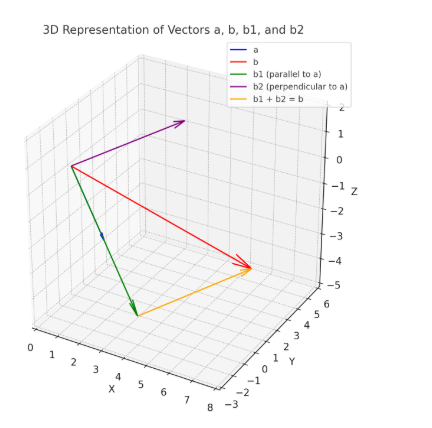
\includegraphics[width=0.6\columnwidth]{../figs/Graph3.png}
\end{center}
\caption{}
\label{fig:Fig}
\end{figure}  
\end{frame}



\begin{frame}[fragile]
    \frametitle{Python Code}
    \begin{lstlisting}
import matplotlib.pyplot as plt
import numpy as np

# Define vectors
a = np.array([2, -1, -2])
b = np.array([7, 2, -3])
b1 = np.array([4, -2, -4])
b2 = np.array([3, 4, 1])

# Function to draw vectors
def draw_vector(ax, start, vec, color, label):
    ax.quiver(*start, *vec, color=color, label=label, arrow_length_ratio=0.1)

# Create 3D plot
fig = plt.figure(figsize=(10,8))
ax = fig.add_subplot(111, projection='3d')

\end{lstlisting}
\end{frame}

\begin{frame}[fragile]
    \frametitle{Python Code}

    \begin{lstlisting}
# Draw from origin
origin = np.array([0,0,0])
draw_vector(ax, origin, a, 'blue', 'a')
draw_vector(ax, origin, b, 'red', 'b')
draw_vector(ax, origin, b1, 'green', 'b1 (parallel to a)')
draw_vector(ax, origin, b2, 'purple', 'b2 (perpendicular to a)')

# Show b as b1 + b2 (parallelogram completion)
draw_vector(ax, b1, b2, 'orange', 'b1 + b2 = b')


    \end{lstlisting}
\end{frame}

\begin{frame}[fragile]
    \frametitle{Python Code}

    \begin{lstlisting}
# Labels and title
ax.set_xlabel('X', fontsize=12)
ax.set_ylabel('Y', fontsize=12)
ax.set_zlabel('Z', fontsize=12)
ax.set_title("3D Representation of Vectors a, b, b1, and b2", fontsize=14)
ax.legend()

# Grid and aspect ratio
ax.grid(True)
ax.set_box_aspect([1,1,1])

# Axis limits
ax.set_xlim(0,8)
ax.set_ylim(-3,6)
ax.set_zlim(-5,2)

# Save figure
plt.savefig("Graph3.png", dpi=300, bbox_inches='tight')
plt.show()




  \end{lstlisting}
\end{frame}

\begin{frame}[fragile]
\frametitle{C Code}
\begin{lstlisting}
#include <stdio.h>

int dotProduct(int a[], int b[], int size) {
    int dot = 0;
    for (int i = 0; i < size; i++) {
        dot += a[i] * b[i];
    }
    return dot;
}

void scalarMultiply(int vector[], int scalar, int result[], int size) {
    for (int i = 0; i < size; i++) {
        result[i] = scalar * vector[i];
    }
}

    \end{lstlisting}

\end{frame}

\begin{frame}[fragile]
\frametitle{C Code}
\begin{lstlisting}
  void vectorSubtract(int a[], int b[], int result[], int size) {
    for (int i = 0; i < size; i++) {
        result[i] = a[i] - b[i];
    }
}

void solve_vectors() {
    int a[3] = {2, -1, -2};
    int b[3] = {7, 2, -3};

    int a_dot_b = dotProduct(a, b, 3);
    int a_dot_a = dotProduct(a, a, 3);

    int k = a_dot_b / a_dot_a;
\end{lstlisting}
\end{frame}
\begin{frame}[fragile]
\frametitle{C Code}
\begin{lstlisting}
   int b1[3];
    scalarMultiply(a, k, b1, 3);

    int b2[3];
    vectorSubtract(b, b1, b2, 3);

    printf("Vector a: [%d, %d, %d]\n", a[0], a[1], a[2]);
    printf("Vector b: [%d, %d, %d]\n", b[0], b[1], b[2]);
    printf("Scalar k: %d\n", k);
    printf("Vector b1 (parallel to a): [%d, %d, %d]\n", b1[0], b1[1], b1[2]);
    printf("Vector b2 (perpendicular to a): [%d, %d, %d]\n", b2[0], b2[1], b2[2]);
}
\end{lstlisting}
\end{frame}


\begin{frame}[fragile]
\frametitle{Python and C Code}

\begin{lstlisting}
import ctypes

# Load the shared object file
lib = ctypes.CDLL('./code.so')

# Call the solve_vectors function (no args, no return)
lib.solve_vectors() 

\end{lstlisting}

\end{frame}

 





\end{document}